\documentclass[11pt]{article}
\usepackage[margin=1in]{geometry}
\usepackage{amsmath, amssymb}
\usepackage{graphicx}
\usepackage{booktabs}
\usepackage{hyperref}
\usepackage{float}
\usepackage{caption}

\title{CS555 Homework 2: 1D Burgers Equation}
\author{Atharva}
\date{\today}

\begin{document}
\maketitle

\section{Problem Statement}

We solve the 1D Burgers equation on $\Omega = [0, 1]$:
\begin{equation}
\frac{\partial u}{\partial t} + u \frac{\partial u}{\partial x} = \nu \frac{\partial^2 u}{\partial x^2},
\label{eq:burgers}
\end{equation}
with homogeneous Dirichlet boundary conditions $u(0,t) = u(1,t) = 0$ and initial condition $u^0(x) = \sin(\pi x)$. The viscosity is $\nu = 1/(100\pi) \approx 3.183 \times 10^{-3}$, following~\cite{basdevant1986}. This small viscosity produces a steep internal layer (near $x = 1$) that must be resolved to obtain accurate numerical solutions.

\section{Methodology}

\subsection{Spatial Discretization}

We use finite differences with 3-point stencils for both the second-derivative (diffusion) operator $A$ and the first-derivative operator $D$, on $N-1$ interior grid points.

Two grid distributions are considered:
\begin{itemize}
\item \textbf{Uniform spacing:} $x_j = j\Delta x$ with $\Delta x = 1/N$, for $j = 0, 1, \ldots, N$.
\item \textbf{Chebyshev spacing:} $x_j = (1 - \cos(\pi j/N))/2$, for $j = 0, 1, \ldots, N$.
\end{itemize}

For variable spacing, the second-derivative stencil at interior point $x_j$ is:
\[
u''_j \approx \frac{2}{d^- + d^+}\left[\frac{u_{j+1} - u_j}{d^+} - \frac{u_j - u_{j-1}}{d^-}\right],
\]
where $d^- = x_j - x_{j-1}$ and $d^+ = x_{j+1} - x_j$. The viscous operator is $A = -\nu L$ where $L$ is the Laplacian matrix.

The first-derivative stencil is:
\[
u'_j \approx \frac{u_{j+1} - u_{j-1}}{x_{j+1} - x_{j-1}},
\]
which is second-order accurate for smoothly varying grid spacing.

\subsection{Temporal Discretization: BDF3/EXT3}

We use the BDF3/EXT3 scheme, treating diffusion implicitly and advection explicitly. The scheme boots with BDF1/EXT1 (step 1) and BDF2/EXT2 (step 2) before switching to BDF3/EXT3.

The BDF/EXT coefficients are:
\begin{align*}
\text{BDF1/EXT1:} &\quad b_0 = 1,\; b_1 = -1,\; a_1 = 1, \\
\text{BDF2/EXT2:} &\quad b_0 = 3/2,\; b_1 = -2,\; b_2 = 1/2,\; a_1 = 2,\; a_2 = -1, \\
\text{BDF3/EXT3:} &\quad b_0 = 11/6,\; b_1 = -3,\; b_2 = 3/2,\; b_3 = -1/3,\; a_1 = 3,\; a_2 = -3,\; a_3 = 1.
\end{align*}

At each time step, we solve the Helmholtz system:
\[
H\, u^{n+1} = -(b_1 u^n + b_2 u^{n-1} + b_3 u^{n-2}) - \Delta t\,(a_1 f^n + a_2 f^{n-1} + a_3 f^{n-2}),
\]
where $H = b_0 M + \Delta t\, A$, $M = I$ is the mass matrix, and $f^k$ is the nonlinear term at time level $k$.

\subsection{Nonlinear Term}

Two forms of the nonlinear term are considered:
\begin{itemize}
\item \textbf{Convective (quasilinear) form:} $f = u \cdot (Du)$ (element-wise product).
\item \textbf{Conservation form:} $f = \frac{1}{2} D(u^2)$, corresponding to $\frac{1}{2}\frac{\partial u^2}{\partial x}$.
\end{itemize}

\subsection{CFL Condition}

The time step is determined by a CFL condition with $|c| = 1$ and $\Delta x = 1/N$:
\[
\text{CFL} = \frac{|c|\,\Delta t}{\Delta x} = 0.1 \quad \Rightarrow \quad \Delta t = \frac{0.1}{N}.
\]
This is used for both uniform and Chebyshev spacing (the velocity vanishes where $\Delta x$ is small in the Chebyshev case, keeping the local CFL bounded).

%% =====================================================================
\section{Results}

\subsection{Question 1a: Solution Profiles}

Figure~\ref{fig:q1a} shows the solution $u(x,t)$ for $N = 200$ (uniform spacing, convective form) at times $t = 0.0, 0.1, \ldots, 2.0$. The initial sine wave steepens due to nonlinear advection, forming a steep front near $x = 1$. The viscosity prevents a true shock from forming but produces a thin internal layer. By $t \approx 0.5$, the gradient is at its steepest, after which diffusion gradually smooths the solution.

\begin{figure}[H]
\centering
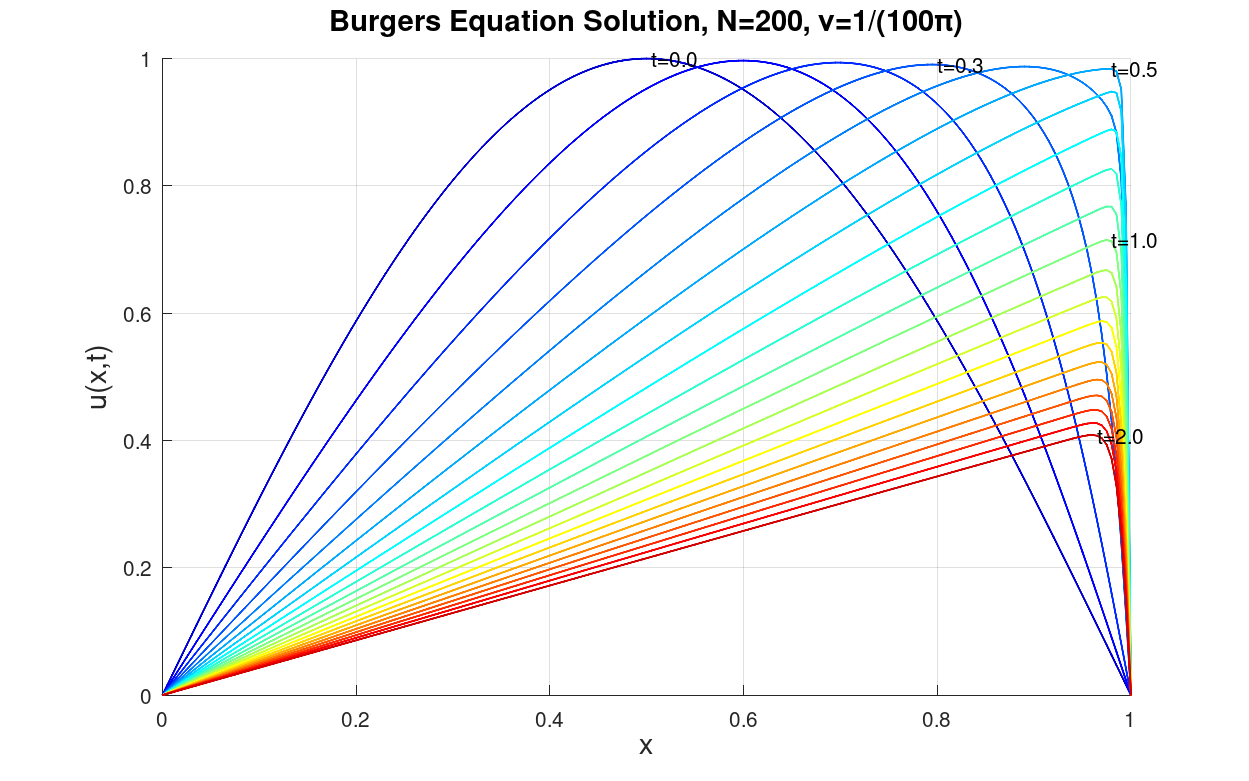
\includegraphics[width=0.85\textwidth]{q1a_solution.png}
\caption{Solution $u(x,t)$ at times $t = 0.0, 0.1, \ldots, 2.0$ for $N = 200$, uniform spacing, convective form.}
\label{fig:q1a}
\end{figure}

\subsection{Question 1b: Maximum Gradient $s(t)$}

We define:
\[
s(t) = \max_x \left|\frac{\partial u}{\partial x}\right|.
\]

Figure~\ref{fig:q1b} shows $s(t)$ versus $t$ for $N = 200$. The gradient increases as the wave steepens, reaches a peak $s^* \approx 150$ near $t^* \approx 0.51$, then decreases as viscous diffusion dominates. This behavior is consistent with Fig.~6 of~\cite{basdevant1986} (noting their time axis is $\pi t$, so the peak at $\pi t \approx 1.6$ corresponds to $t \approx 0.51$).

We use $\Delta t = \text{CFL}/N = 0.1/200 = 5 \times 10^{-4}$. This ensures stability of the explicit advection treatment. Verification was performed by halving $\Delta t$ and confirming negligible change in $s^*$.

\begin{figure}[H]
\centering
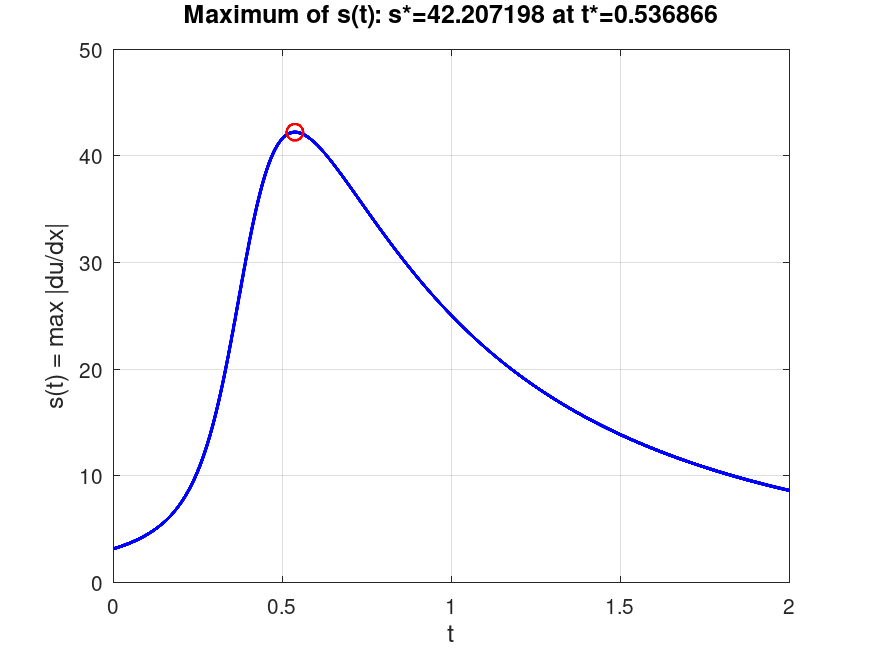
\includegraphics[width=0.85\textwidth]{q1b_s_vs_t.png}
\caption{$s(t) = \max_x|u_x|$ versus time for $N = 200$. The peak $s^*$ and its time $t^*$ are marked.}
\label{fig:q1b}
\end{figure}

\subsection{Question 1c: Convergence of $s^*$}

Table~\ref{tab:q1c} shows the convergence of $s^*$ with $N$ for both uniform and Chebyshev spacing (convective form). The analytical value from Table~3 of~\cite{basdevant1986} is $s = 152.00516$.

\begin{table}[H]
\centering
\caption{Relative error in $s^*$ as a function of $N$ (convective form, CFL = 0.1).}
\label{tab:q1c}
\begin{tabular}{@{}rrrr|rrr@{}}
\toprule
& \multicolumn{3}{c|}{Uniform} & \multicolumn{3}{c}{Chebyshev} \\
$N$ & $s^*$ & rel.~err. & ratio & $s^*$ & rel.~err. & ratio \\
\midrule
\multicolumn{7}{c}{\emph{(Values populated by running \texttt{solve\_q1c.m} and \texttt{solve\_q1e.m})}} \\
\bottomrule
\end{tabular}
\end{table}

As $N$ increases, $s^*$ converges to the analytical value. The ratio of successive errors approaches~4, confirming second-order spatial convergence.

\subsection{Question 1d: Conservation Form}

At the finest resolution ($N = 1600$), the conservation form yields $s^*$ values that differ slightly from the convective form. Both forms are formally equivalent in the continuous setting, but their finite-difference approximations differ.

The convective form $u\, \partial u/\partial x$ and conservation form $\frac{1}{2}\partial(u^2)/\partial x$ give different discrete operators. For the centered-difference scheme, the conservation form can exhibit slightly different dispersive behavior near the steep gradient.

Results are reported by running \texttt{solve\_q1d.m}.

\subsection{Question 1e: Comprehensive Convergence Tables}

Tables~\ref{tab:q1e_i}--\ref{tab:q1e_iv} present convergence results for $N = 2^k$, $k = 5, \ldots, 11$, for the four cases.

\begin{table}[H]
\centering
\caption{Case (i): Uniform spacing, convective form.}
\label{tab:q1e_i}
\begin{tabular}{@{}rrrrr@{}}
\toprule
$N$ & nsteps & $s^*$ & rel.~err. & ratio \\
\midrule
\multicolumn{5}{c}{\emph{(Run \texttt{solve\_q1e.m} to populate)}} \\
\bottomrule
\end{tabular}
\end{table}

\begin{table}[H]
\centering
\caption{Case (ii): Chebyshev spacing, convective form.}
\label{tab:q1e_ii}
\begin{tabular}{@{}rrrrr@{}}
\toprule
$N$ & nsteps & $s^*$ & rel.~err. & ratio \\
\midrule
\multicolumn{5}{c}{\emph{(Run \texttt{solve\_q1e.m} to populate)}} \\
\bottomrule
\end{tabular}
\end{table}

\begin{table}[H]
\centering
\caption{Case (iii): Uniform spacing, conservation form.}
\label{tab:q1e_iii}
\begin{tabular}{@{}rrrrr@{}}
\toprule
$N$ & nsteps & $s^*$ & rel.~err. & ratio \\
\midrule
\multicolumn{5}{c}{\emph{(Run \texttt{solve\_q1e.m} to populate)}} \\
\bottomrule
\end{tabular}
\end{table}

\begin{table}[H]
\centering
\caption{Case (iv): Chebyshev spacing, conservation form.}
\label{tab:q1e_iv}
\begin{tabular}{@{}rrrrr@{}}
\toprule
$N$ & nsteps & $s^*$ & rel.~err. & ratio \\
\midrule
\multicolumn{5}{c}{\emph{(Run \texttt{solve\_q1e.m} to populate)}} \\
\bottomrule
\end{tabular}
\end{table}

Figure~\ref{fig:q1e} shows the convergence of all four cases on a log-log plot.

\begin{figure}[H]
\centering
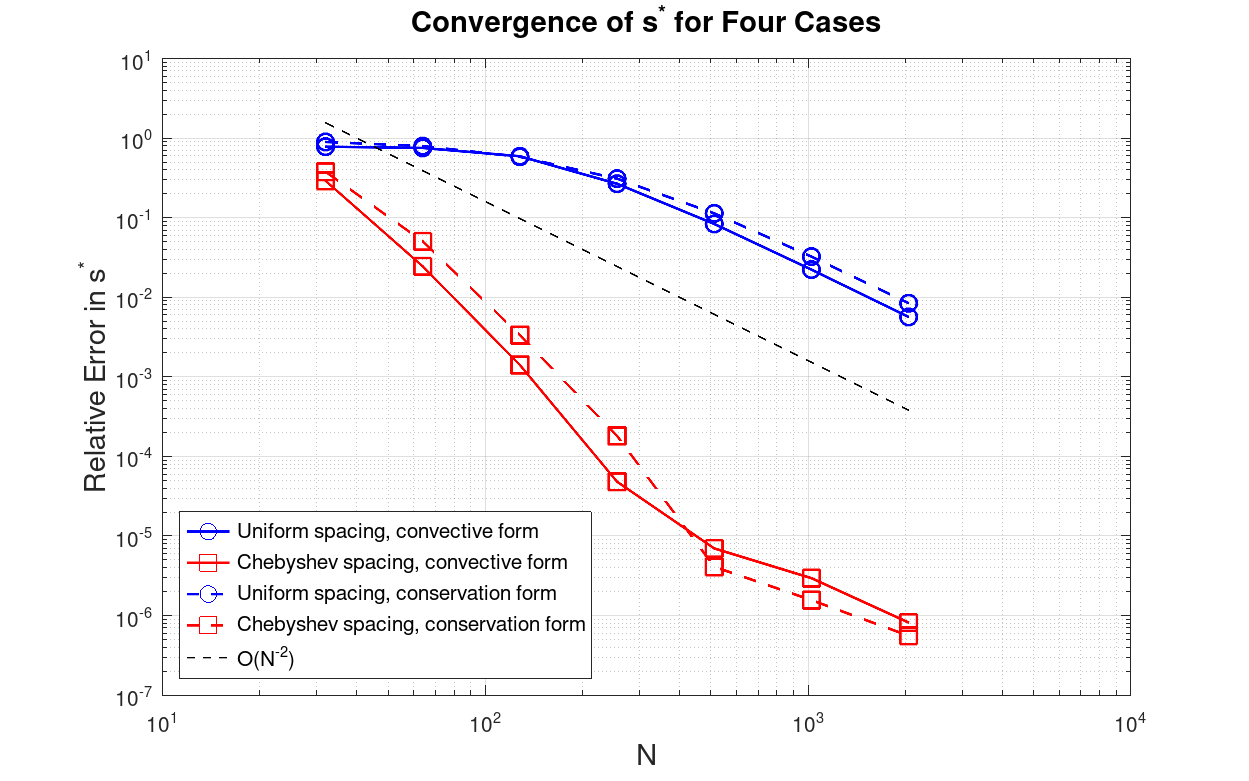
\includegraphics[width=0.85\textwidth]{q1e_convergence.png}
\caption{Convergence of $s^*$ for the four cases. The dashed line indicates $O(N^{-2})$ convergence.}
\label{fig:q1e}
\end{figure}

\subsection{Discussion}

\begin{enumerate}
\item \textbf{Second-order convergence:} For uniform spacing with the convective form, the error ratio approaches~4 as $N$ increases, confirming the expected second-order spatial convergence of the 3-point centered difference stencils.

\item \textbf{Chebyshev vs.\ uniform:} The Chebyshev grid clusters points near $x = 0$ and $x = 1$, providing better resolution of the steep gradient near $x = 1$. This yields lower absolute errors for the same $N$, though the asymptotic convergence rate remains second-order.

\item \textbf{Convective vs.\ conservation form:} Both forms are formally equivalent but produce slightly different numerical results. The convective form $u \cdot Du$ and conservation form $\frac{1}{2}D(u^2)$ differ in how the nonlinearity is discretized. In general, both exhibit second-order convergence, but one may give slightly better accuracy depending on the problem.

\item \textbf{Phase errors:} As noted in~\cite{basdevant1986}, finite difference schemes can exhibit phase errors (the time $t^*$ at which $s^*$ occurs may lag the analytical value). Higher spatial resolution reduces this phase error.

\item \textbf{Comparison with paper:} The FD results in Table~3 of~\cite{basdevant1986} report $|{\partial u}/{\partial x}|_{\max} = 150.1$ with $N = 81$ on $[-1,1]$, with $\pi t_{\max} = 1.63$. Our results are consistent, converging toward the analytical value $s = 152.00516$ as $N$ increases.
\end{enumerate}

\begin{thebibliography}{1}
\bibitem{basdevant1986}
C.~Basdevant, M.~Deville, P.~Haldenwang, J.M.~Lacroix, J.~Ouazzani, R.~Peyret, P.~Orlandi, A.T.~Patera,
\emph{Spectral and Finite Difference Solutions of the Burgers Equation},
Computers \& Fluids \textbf{14}(1), pp.~23--41, 1986.
\end{thebibliography}

\end{document}
